\chapter{Results}  %Title of the First Chapter

\ifpdf
    \graphicspath{{Chapter1/Figs/Raster/}{Chapter1/Figs/PDF/}{Chapter1/Figs/}}
\else
    \graphicspath{{Chapter1/Figs/Vector/}{Chapter1/Figs/}}
\fi



\section{Frequency Splittings due to Differential Rotation} %Section - 1.1 
In this treatment we show that while taking very closely spaced multiplets, the isolated multiplet condition breaks down and there is significant cross coupling across modes due to differential rotation alone. Because axis symmetry imposes the $m'=m$ selection rule, the supermatrix $Z_{k'k}$ of perturbation $\dLd$ is a sparse matrix consisting of diagonals and subdiagonal as show in figure (\ref{fig:coup_mat}). As a case study, we choose to investigate the splitting coefficients of the mode $\mode{0}{77}$ as a result of cross coupling with its neighbouring modes which all lie withing an interval of $100\mu Hz$.

\subsection{Splitting with pure rotation}
We plot the split frequencies $\mode{0}{77}$ along with some neighbouring modes to contrast the results obtained from a dpt and a qdpt analysis.

\begin{figure}[h!]
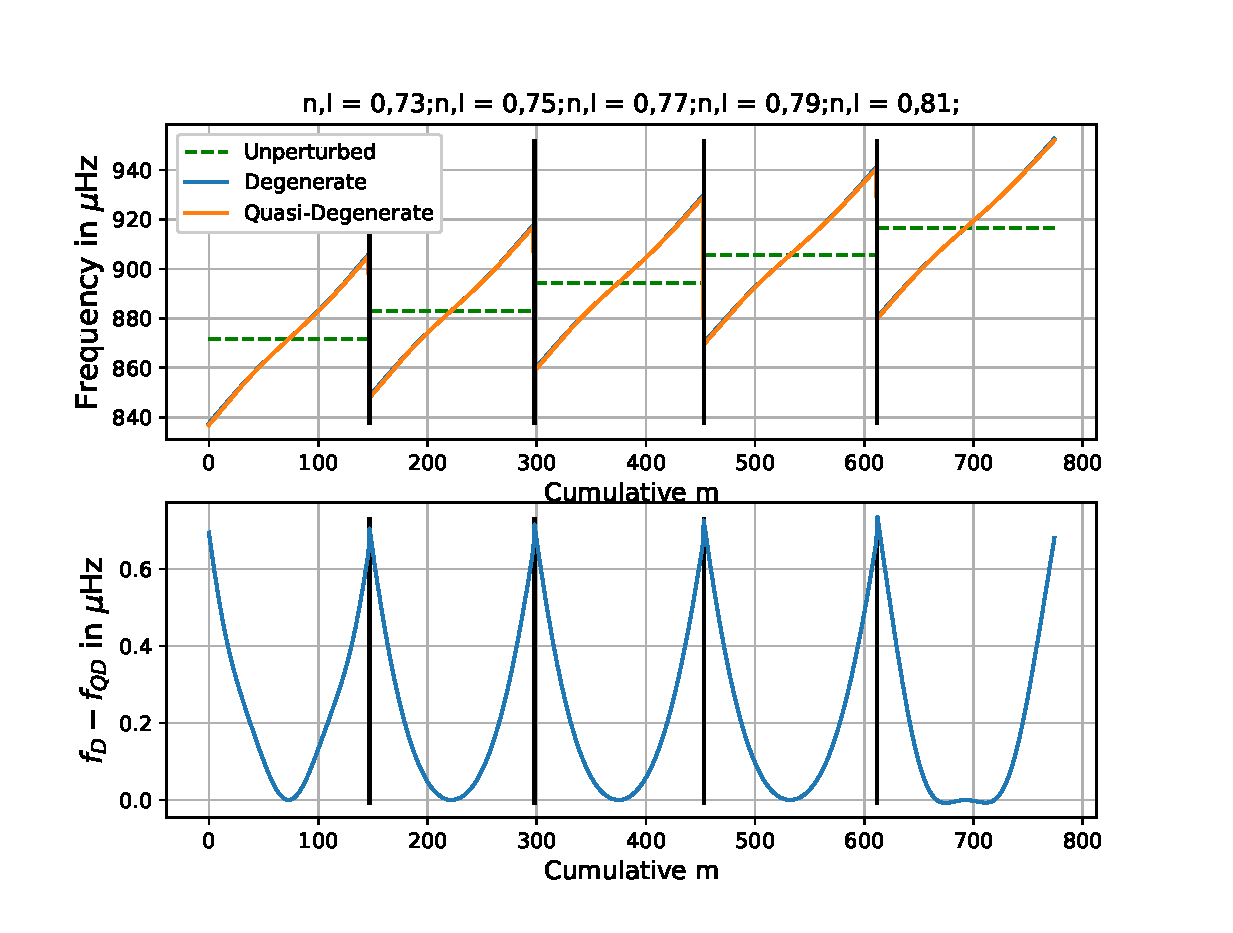
\includegraphics[scale=0.8,center]{Chapter4/figs/dr_split}
\caption{Dpt and Qdpt splits with $\mode{0}{73}$, $\mode{0}{75}$, $\mode{0}{77}$, $\mode{0}{79}$, and $\mode{0}{81}$ which have frequencies 871.63$\mu Hz$, 883.12$\mu Hz$, 894.43$\mu Hz$, 905.62$\mu Hz$, and 916.66$\mu Hz$ respectively. Top plot shows frequency splittings of the five modes and their unperturbed frequencies. Bottom plot shows the departure of the qdpt frequencies from the dpt frequencies.}
\label{fig:split_dr}
\end{figure}

A coefficients obtained from the split is tabulated

\begin{table}

\begin{tabular}{|l|c|r|}
\hline
4.64e-310 & 4.64e-310 & 6.91e-310 \\ \hline
6.91e-310 & 4.75e-309 & 1.64e-287 \\
\hline
\end{tabular}
\end{table}

\subsection{Splitting with pure rotation removed}
After removing a constant 440nHz from the $w_1^0/r$ rotational profile, we get the following splitting of frequencies for dpt and qdpt respectively as shown in \ref{fig:split_dr}. Qdpt is performed taking 5 modes all lying in a band of width $100\mu Hz$.
\begin{figure}[h!]
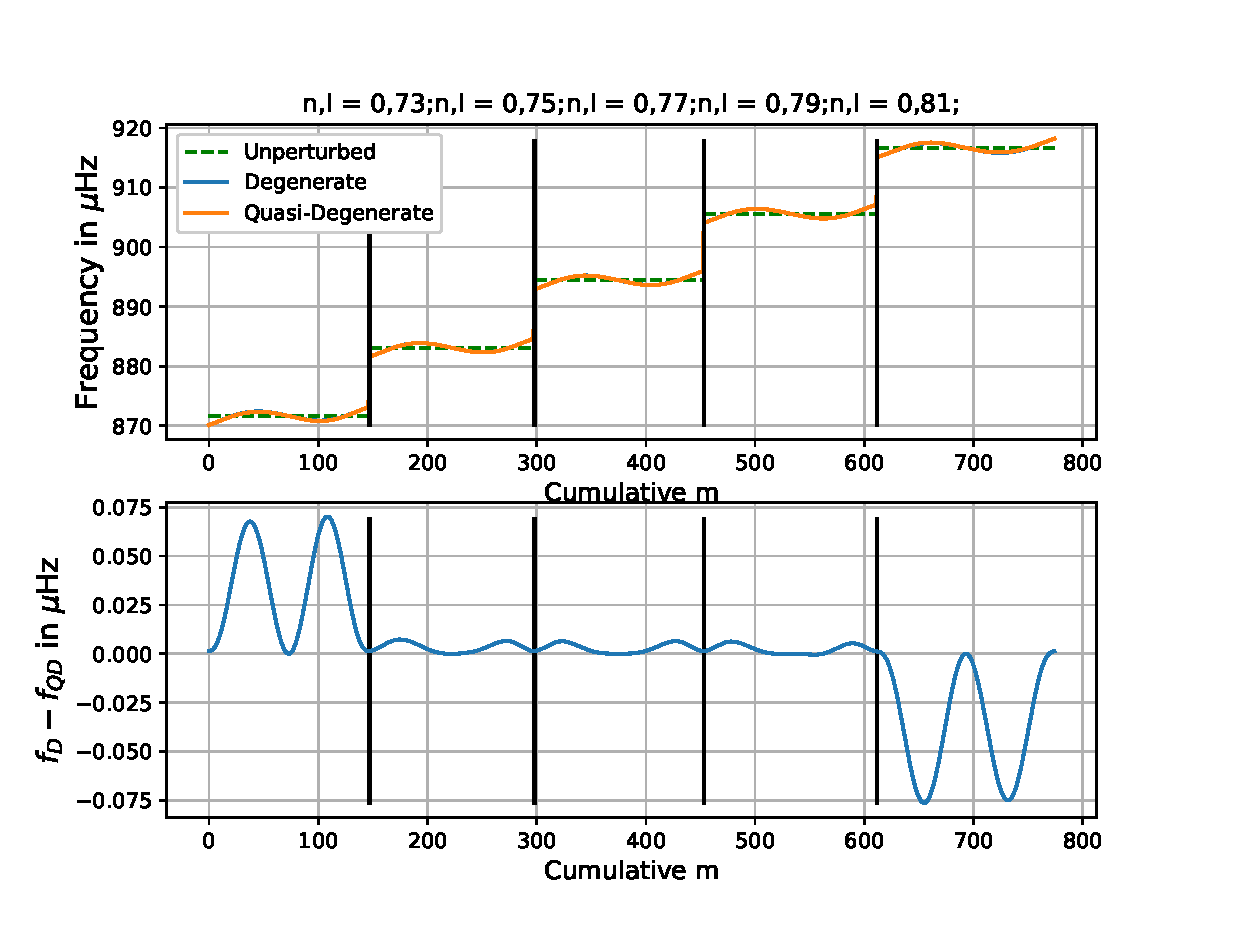
\includegraphics[scale=0.8,center]{Chapter4/figs/dr_split_rm}
\caption{Dpt and Qdpt splits with $440 nHz$ removed from $w_1^0$ for modes $\mode{0}{73}$, $\mode{0}{75}$, $\mode{0}{77}$, $\mode{0}{79}$, and $\mode{0}{81}$ which have frequencies 871.63$\mu Hz$, 883.12$\mu Hz$, 894.43$\mu Hz$, 905.62$\mu Hz$, and 916.66$\mu Hz$ respectively. Top plot shows frequency splittings of the five modes and their unperturbed frequencies. Bottom plot shows the departure of the qdpt frequencies from the dpt frequencies.}
\label{fig:split_dr_rm}
\end{figure}

\subsection{QDPT vs DPT with increasing coupling modes}

\begin{figure}[h!]
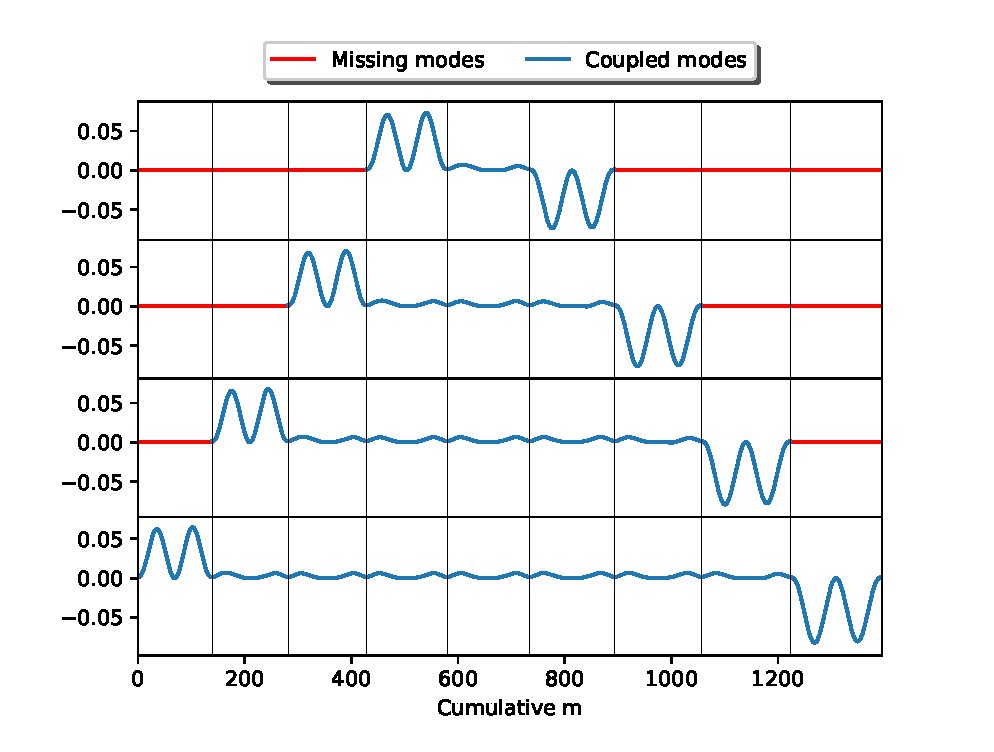
\includegraphics[scale=0.9, center]{Chapter4/figs/qdpt_err}
\caption{Shows the difference between frequencies obtained from qdpt and dpt when different number of neighbouring modes are allowed to couple. From top it shows $\mode{0}{77}$ coupling with two, four, six, and eight closest $\Delta l=2$ neighbours as listed in table}
\label{fig:qdpt_err}
\end{figure}

\section{Splittings due to Lorentz Stresses} %Section - 1.2
